%-%-%-%-%-%-%-%-%-%-%-%-%-%-%-%-%-%-%-%-%-%-%-%-%-%
% EE531: laboratório de Eletrônica Básica I       %  
% Experimento 2: Diodos                           %
% Data:20/08/2010                                 %
% Unicamp,Campinas,São Paulo,Brasil               % 
% Grupo:                                          %
%       - Daniel Lins Mattos                      %
%       - Raquel Mayumi Kawamoto                  %
%       - Tiago Chedraoui Silva                   % 
%-%-%-%-%-%-%-%-%-%-%-%-%-%-%-%-%-%-%-%-%-%-%-%-%-%
%\documentclass[letter]{article}  % formato impressao IC
\documentclass[a4paper]{article} % formato impressao FEEC

%%% fontes %%%
\usepackage[T1]{fontenc}
\usepackage[brazil]{babel}    % dá suporte para os termos na língua portuguesa do Brasi
\usepackage[utf8]{inputenc}   % acentuação
\usepackage{ae,aecompl,aeguill}       % pdfs mais bonitos =)

%%% outros %%%
\usepackage{multirow}
\usepackage{textcomp}
\usepackage{color}       
\usepackage{indentfirst}      % retira padrao americano de paragrafos
\usepackage{multicol}   
\usepackage[linkbordercolor={1 1 1},urlcolor=black,colorlinks=true]{hyperref} % links
\usepackage{subfig}
\usepackage[letterpaper]{geometry}
\geometry{verbose,lmargin=3cm,rmargin=3cm}

% circuito eletrico
\usepackage{electComp}
\usetikzlibrary{decorations,decorations.pathmorphing,decorations.pathreplacing}
\usepackage{verbatim}
\usepackage{pstricks}
\usepackage{boxdims}


\date{Setembro 10, 2010}
% Capa estilizada %
\newcommand*{\titleTMB}{\begingroup \centering \settowidth{\unitlength}{\LARGE EE531} {\large\scshape EE531 - Turma S}\\[0.2\baselineskip] \rule{11.0cm}{1.6pt}\vspace*{-\baselineskip}\vspace*{2pt} \rule{11.0cm}{0.4pt}\\[\baselineskip] {\LARGE  Diodos}\\\vspace*{\baselineskip}  {\itshape Laboratório de Eletrônica Básica I - Segundo Semestre de 2010}\\ \rule{11.0cm}{0.4pt}\vspace*{-\baselineskip}\vspace{3.2pt} \rule{11.0cm}{1.6pt}\\[\baselineskip] {\large\scshape Professor: José Cândido Silveira Santos Filho}\par \vfill {\normalsize   \scshape 
    \begin{center} 
      \begin{tabular}{  l  l  p{5cm} } 
 	Daniel Lins Mattos & RA: 059915\\
        Raquel Mayumi Kawamoto & RA: 086003\\
        Tiago Chedraoui Silva  & RA: 082941\\
      \end{tabular} \end{center}
    \itshape 10 de setembro de 2010    }\\[\baselineskip] \vspace{3.2pt} \endgroup}


\begin{document}
\titleTMB 
\newpage


Para este experimento da disciplina de laboratório de eletrônica básica I, tem-se como objetivo caracterizar diodos semicondutores, familiarizar-se com seus principais parâmetros e realizar circuitos que os possuam.As ferramentas utilizadas são a fonte de alimentação dual, um gerador de funções e um osciloscópio digital. Para este presente experimento utilizam-se ainda um protoboard, dois resistores de 
$10k\Omega$, um resistor de $1k\Omega$ três capacitores eletrolíticos de de $100\mu$F, oito diodos 1n4001, dois diodos 1N4148, um amplificador operacional 741 e um tranformador de 110 $V_{ac}$,9 $V_{ac}$. 



\section*{Parte Experimental}
%\begin{enumerate}
%\item
1. Para esta parte inicial do experimento, o gerador de funções é ajustado para produzir um sinal de tensão com sua forma de onda triangular, com amplitude 10$V_{pp}$, com offset de $5V$, frequência de $10kHz$ e simetria de 50\%. 

Além disso, o circuito da figura \ref{circ:1} --- composto de um amplificador operacional 741, um resistor (R$_i$) de $1k\Omega$, e dois diodos 1n4148 (D$_1$ e D$_2$) --- é montado e o canal um do osciloscópio é colocado entre D$_1$ e R$_i$ e o canal dois na saída do amplificador operacional. 

 É importante que a onda gerada seja positiva, pois caso fosse negativa diodo $D_1$ atuaria bloquearia o sinal, logo o amplificador operacional saturaria.

\vspace{3mm}
\begin{figure}[h]
\centerline{\input circ1.tex}
\caption{Circuito para caracterização V versus I do diodo \label{circ:1}}
\end{figure}

Supondo que o amplificador operacional seja ideal, nenhuma corrente de entrada é drenada, ou seja, a corrente $i$ caracterizada em $D_1$ e $R_i$ é a mesma que em $D_2$. Além disso, a tensão entre o terminal de saída e o terra é equivalente a $A(v_2-v_1)$, sendo o ganho $A$ idealmente infinito. Logo, tem-se que:
\begin{equation}
\frac{V_D}{A}=(v_2-v_1)\approx0
\end{equation}

Como $v_1=0$ temos que $v_2=0$, assim:.
\begin{equation}
i=\frac{V_{CH2}}{R_{i}}\\
\end{equation}

Utilizando o canal 1, tem-se que:  
\begin{equation}
V_D=-V_{CH1}\\
\end{equation}


%\begin{figure}[h!]
%\begin{centering}
%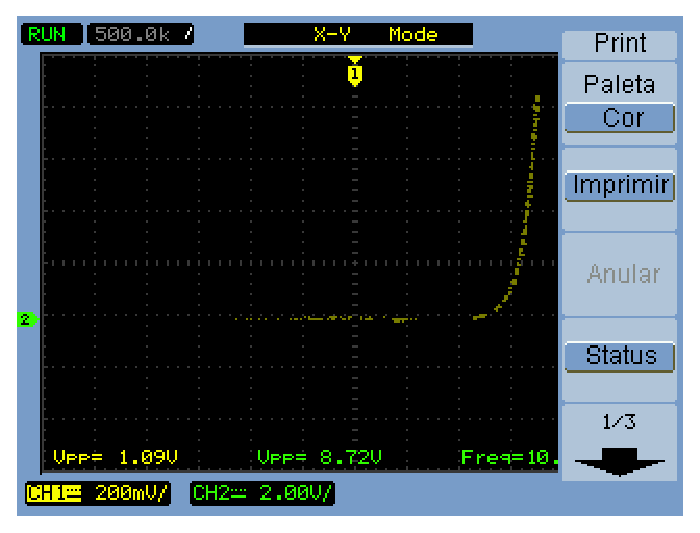
\includegraphics[scale=0.7]{Imagens/3.1/q1} \caption{Curva característica V versus I do diodo \label{fig:q1-curva}}
%\par\end{centering}
%\end{figure}

\newpage
Utilizando o recurso Time Base X-Y do osciloscópio, obtemos uma curva caracterísica (V versus I) do diodo presente na figura \ref{fig:q1-curva2}. As escala do eixo $V_D$ vale $500mV$/célula. Portanto, o diodo em condução direta apresenta um queda de tensão de aproximadamente $0,7V$.    
\begin{figure}[h]
\begin{centering}
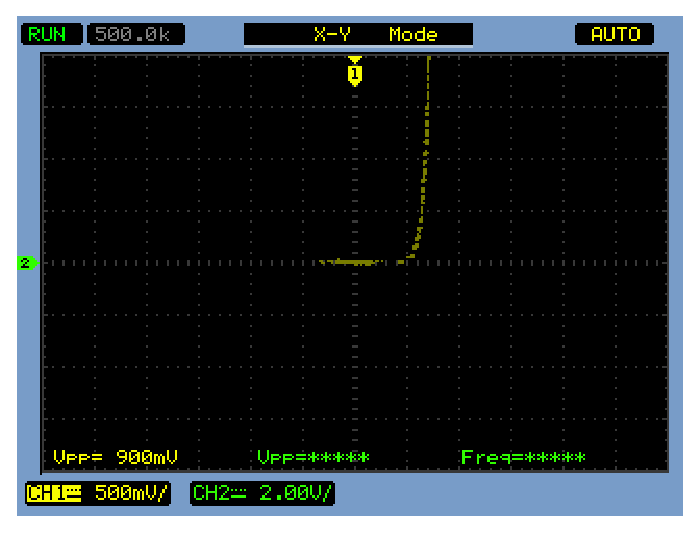
\includegraphics[scale=0.7]{Imagens/3.1/NewFile0} \caption{Curva característica V versus I do diodo  \label{fig:q1-curva2}}
\par\end{centering}
\end{figure}


\begin{figure}[h]
\begin{centering}
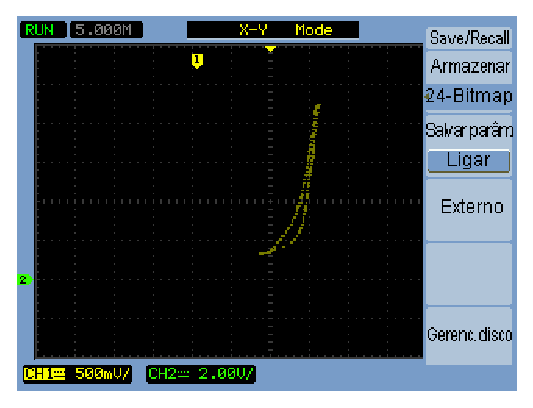
\includegraphics[scale=1.0]{Imagens/3.1.opcional/opcio} \caption{Curva de histerese \label{fig:q1-his}}
\par\end{centering}
\end{figure}


\newpage

\vspace{3mm}
\begin{figure}[h]
\centerline{\input circ2.tex}
\caption{Circuito retificador de meia onda \label{tab:circ}}
\end{figure}


\vspace{3mm}
\begin{figure}[h]
\centerline{\input circ3.tex}
\caption{Circuito retificador de onda completa  \label{tab:circ}}
\end{figure}


\vspace{3mm}
\begin{figure}[h]
\centerline{\input circ4.tex}
\caption{Duplicador de tensão \label{tab:circ}}
\end{figure}


\newpage
\begin{figure}[h!]
\begin{centering}
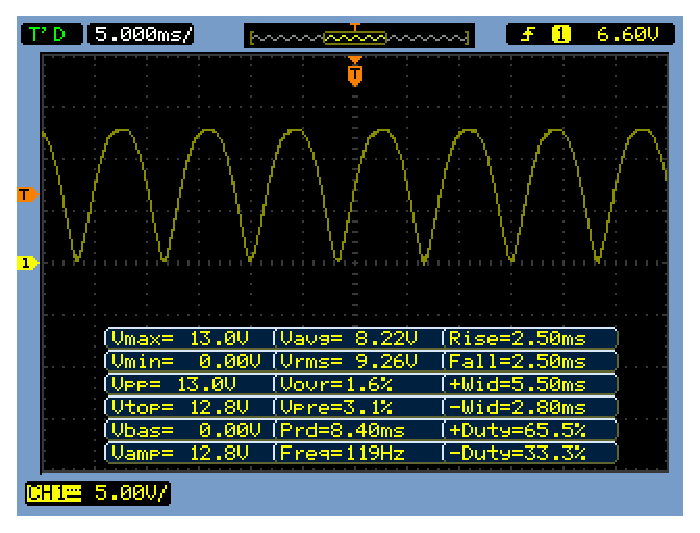
\includegraphics[scale=0.7]{Imagens/3.3.1onda_completa/3} \caption{Medida da tensão no nó 3 \label{fig:q2-no3}}
\par\end{centering}
\end{figure}



\begin{figure}[h!]
\begin{centering}
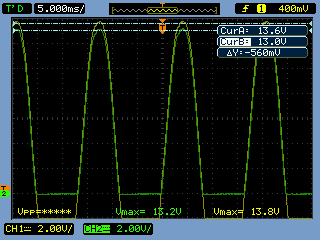
\includegraphics[scale=0.7]{Imagens/3.3.1onda_completa/31} \caption{Medida da tensão diferencial entre os nós 2 e 3 \label{fig:Fig-45}}
\par\end{centering}
\end{figure}


\begin{figure}[h!]
\begin{centering}
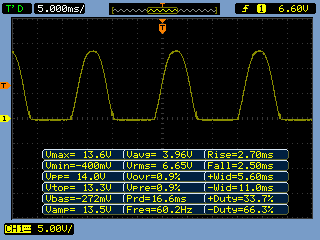
\includegraphics[scale=0.7]{Imagens/3.3.1onda_completa/no1} \caption{Medida da tensão no nó 1 \label{fig:q2-no1}}
\par\end{centering}
\end{figure}

\newpage
\begin{figure}[h!]
\begin{centering}
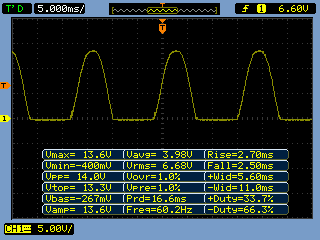
\includegraphics[scale=0.7]{Imagens/3.3.1onda_completa/no2} \caption{Medida da tensão no nó 2  \label{fig:q2-no2}}
\par\end{centering}
\end{figure}


\begin{figure}[h!]
\begin{centering}
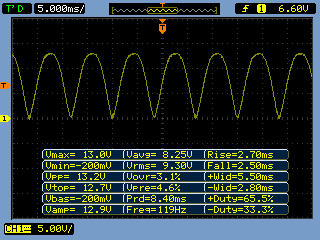
\includegraphics[scale=0.7]{Imagens/3.3.1onda_completa/no3} \caption{Medida da tensão diferencial entre os nós 2 e 3 \label{fig:Fig-45}}
\par\end{centering}
\end{figure}


\begin{figure}[h!]
\begin{centering}
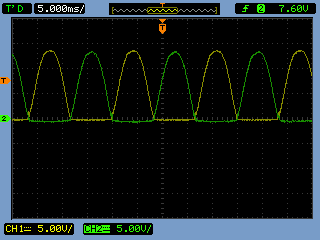
\includegraphics[scale=0.7]{Imagens/3.3.1onda_completa/no12} \caption{Medida da tensão nos nós 1 e 2 \label{fig:Fig-45}}
\par\end{centering}
\end{figure}


\begin{figure}[h!]
\begin{centering}
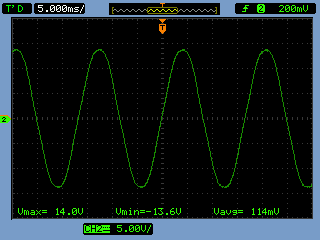
\includegraphics[scale=0.7]{Imagens/3.3.1onda_completa/p1q3} \caption{Medida da tensão diferencial entre os nós 2 e 3 \label{fig:Fig-45}}
\par\end{centering}
\end{figure}



\newpage
\begin{figure}[h!]
\begin{centering}
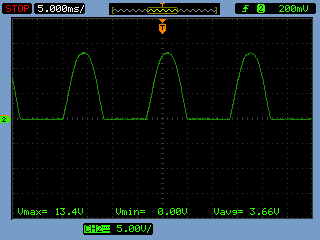
\includegraphics[scale=0.7]{Imagens/3.3.1onda_completa/p2q3} \caption{Medida da tensão diferencial entre os nós 2 e 3 \label{fig:Fig-45}}
\par\end{centering}
\end{figure}

\begin{figure}[h!]
\begin{centering}
\includegraphics[scale=0.7]{Imagens/3.3.1ret_meia_onda/311} \caption{Medida da tensão diferencial entre os nós 2 e 3 \label{fig:Fig-45}}
\par\end{centering}
\end{figure}

\begin{figure}[h!]
\begin{centering}
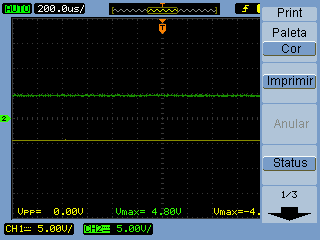
\includegraphics[scale=0.7]{Imagens/3.4duplicador_tensao/423} \caption{Medida da tensão diferencial entre os nós 2 e 3 \label{fig:Fig-45}}
\par\end{centering}
\end{figure}


\newpage
\begin{figure}[h!]
\begin{centering}
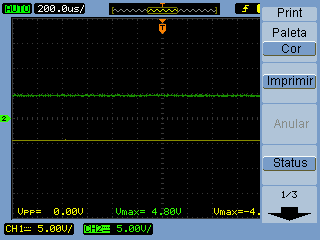
\includegraphics[scale=0.7]{Imagens/3.4duplicador_tensao/423} \caption{Tensão de saída nos nós 1 e 2 \label{fig:q4-no12}}
\par\end{centering}
\end{figure}


\begin{figure}[h!]
\begin{centering}
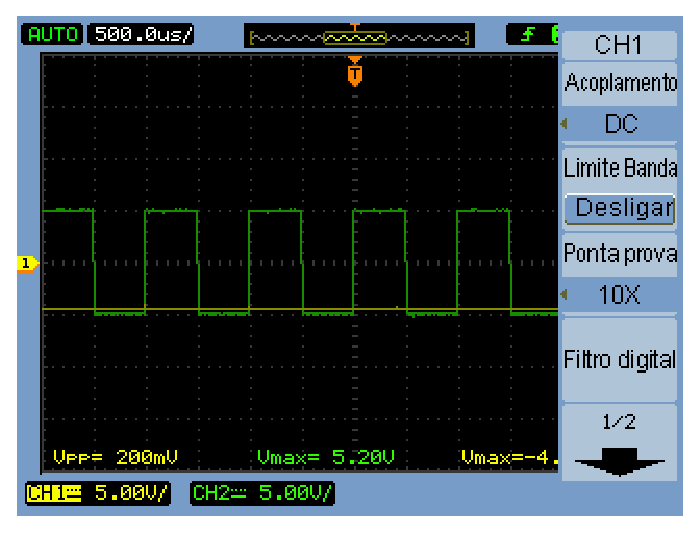
\includegraphics[scale=0.7]{Imagens/3.4duplicador_tensao/444} \caption{Análise do sinal de saída no nó x \label{fig:q4-no}}
\par\end{centering}
\end{figure}


\begin{figure}[h!]
\begin{centering}
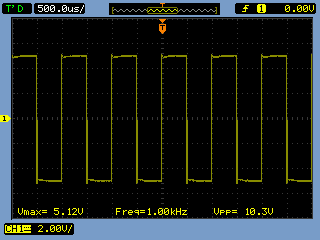
\includegraphics[scale=0.7]{Imagens/3.4duplicador_tensao/Vin} \caption{Onda de entrada do circuito\label{fig:q4-vin}}
\par\end{centering}
\end{figure}



\begin{figure}[h!]
\begin{centering}
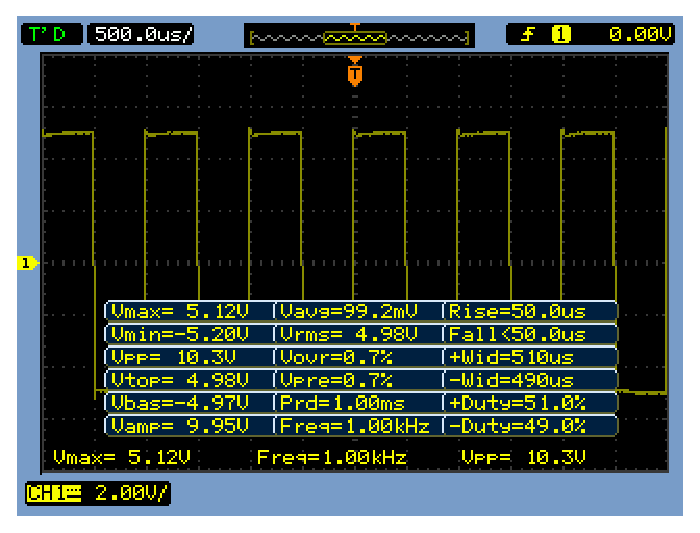
\includegraphics[scale=0.7]{Imagens/3.4duplicador_tensao/Vinmedidas} \caption{Medidas da onda de entrada do circuito \label{fig:q4-vindata}}
\par\end{centering}
\end{figure}


\newpage
\begin{figure}[h!]
\begin{centering}
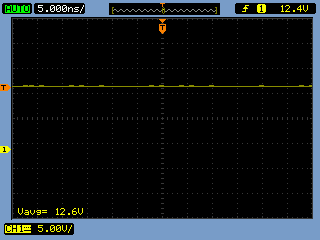
\includegraphics[scale=0.7]{Imagens/3.3.4capacitor_paralelo/3cao1} \caption{Característica onda após a inserção de capacitor em paralelo \label{fig:Fig-45}}
\par\end{centering}
\end{figure}


\begin{figure}[h!]
\begin{centering}
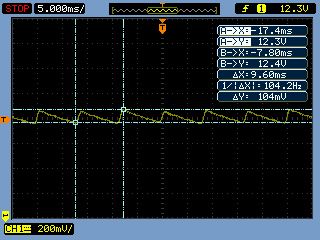
\includegraphics[scale=0.7]{Imagens/3.3.4capacitor_paralelo/3cap} \caption{Aproximação da imagem da onda após a inserção de capacitor em paralelo \label{fig:q2-cap}}
\par\end{centering}
\end{figure}


\end{document}
